\documentclass[journal]{./IEEEtran}
\usepackage{cite,graphicx}
\usepackage{float}
\usepackage{array}
\usepackage{url}
\usepackage{amsmath,amssymb}
\setlength{\parskip}{0.5em}  % space between paragraphs
\newcommand{\SPTITLE}{NoEsc: A Comparative Analysis of Heuristic and Machine Learning-Based Detection of Host-Based Privilege Escalation on Linux
}
\newcommand{\ADVISEE}{Klenn Jakek V. Borja}
\newcommand{\ADVISER}{Joseph Anthony C. Hermocilla}

\newcommand{\BSCS}{Bachelor of Science in Computer Science}
\newcommand{\ICS}{Institute of Computer Science}
\newcommand{\UPLB}{University of the Philippines Los Ba\~{n}os}
\newcommand{\REMARK}{\thanks{Presented to the Faculty of the \ICS, \UPLB\
                             in partial fulfillment of the requirements
                             for the Degree of \BSCS}}
        
\markboth{CMSC 190 Special Problem, \ICS}{}
\title{\SPTITLE}
\author{\ADVISEE~and~\ADVISER%
\REMARK
}

%%%%%%%%%%%%%%%%%%%%%%%%%%%%%%%%%%%%%%%%%%%%%%%%%%%%%%%%%%%%%%%%%%%%%%%%%%

\begin{document}

% TITLE
\maketitle

% ABSTRACT
% INDEX TERMS
% INTRODUCTION
\section{Introduction}

\subsection{Background of the Study}
The use of Linux systems in critical infrastructure has been widespread, from university machines (like in ICS laboratories) to cloud systems. Due to its prevalence, the need to secure these systems against unauthorized access increases to such an extent that it becomes a necessity.

Privilege Escalation, one example of gaining unauthorized access to a system, is  the process by which an attacker with low-level access elevates their privileges, typically to gain \texttt{root} access \cite{happe2024}. Students in the university, by the time they operate the machines, already have low-level access to the systems. It is only a matter of time whether a person with malicious intent gains unauthorized access that may lead to credential stealing and propagation across the university network \cite{schroder2025}. 

Host-Based Intrusion Detection (or HIDS) is a detection system which monitors the internal activities of a single machine by analyzing its system logs \cite{shin2020}. One common and powerful technique used by HIDS on Linux is the analysis of system call traces \cite{shin2020}. 

The Linux Audit System, also called \textit{auditd}, is a built-in framework on Linux that collects these detailed system call traces \cite{groenewoud2024}. It is deemed a foundational and industry-standard tool for "detection engineering" which are used by security engineers \cite{groenewoud2024}.

Once data are collected, two primary methodologies exist for its analysis. First, is the heuristic rule-based approach, which uses simple, human-written \texttt{IF-THEN} rules to identify malicious behavior \cite{liu2021}. The key advantage of this method is its interpretability \cite{liu2021}. Second, is the machine learning approach, which is described as data-driven where a model learns to differentiate between benign and malicious patterns in the dataset. 

Within the machine learning domain, a key challenge is the trade-off between model interpretability and performance. While ensemble methods like Random Forest (RF) are often cited for their potential interpretability, they can still be regarded as ``black boxes'' due to their complexity \cite{pereira2018}. Consequently, selecting a machine learning model involves balancing the need for high detection accuracy against the inherent opacity of the algorithm.

\subsection{Statement of the Problem}
Securing Linux systems in academic environments, like UPLB ICS laboratories, against privilege escalation remains unresolved. Although HIDS are considered to be the lead solution to this problem, selecting the right methodology remains a challenge.

This comparative study faces a trade-off: traditional heuristic rule-based systems are interpretable, extensible, and of crucial importance to an administrator for validating an alert, but are usually rigid and can be bypassed by novel attacks and edge cases. Furthermore, ML models have achieved superior performance in detecting the anomalous behavior of the system; however, its “black box” nature whose decisions are opaque and therefore untrustworthy, or hardly interpretable by an administrator.

However, the effectiveness of either a rule-based or an ML approach is not guaranteed; both must be specifically designed to be effective against modern threats. While simple rule-based tools like \texttt{rkhunter} and \texttt{chkrootkit} have existed for years, a recent comprehensive analysis by Stühn et al. in "The Hidden Threat" concluded that many of these tools are now "insufficient" and have significant detection gaps \cite{stuhn2024}. This is especially true for the common misconfiguration-based privilege escalation vectors cataloged in the "Got Root?" benchmark, which are often missed by traditional signature-based tools \cite{happe2024}. Similarly, an ML-based approach is only as effective as the features it is trained on; a model relying on simplistic features would likely fail to distinguish these same subtle attack patterns from benign administrative activity.

It is yet unclear whether the interpretability of rule-based systems or the accuracy of machine learning models is preferable for a practical and lightweight security tool suitable for an academic environment. This study addresses the gap using comparative analysis to determine the feasibility and effectiveness of these two opposing methodologies in a real-world academic setting.

Specifically, this study aims to answer the following questions:
\begin{enumerate}
    \item How effective is a heuristic rule-based engine compared to a machine learning-based engine in detecting privilege escalation attacks in terms of detection rate and false positives?
    \item What is the performance overhead incurred by the detection system when utilizing these two different detection methodologies?
    \item What are the specific trade-offs between the interpretability of the rule-based approach and the accuracy of the SVM-based approach in the context of an academic laboratory environment?
\end{enumerate}

\subsection{Significance of the Study}
The study's primary contribution will be a working prototype of a lightweight, host-based intrusion detector specifically designed for environments like the ICS computer labs. The study provides a necessary layer of security for Linux systems that students use daily. By focusing on common privilege escalation vectors, the prototype will be able to address high-impact threats in a more efficient manner.

The study will provide empirical data on the trade-off between interpretability and accuracy of the two engines where its findings will help inform future design on security tools in addressing which methodology is better suited for such security challenges.

\subsection{Objectives of the Study}
The aim of this research is to design, implement, and comparatively evaluate two distinct methodologies for the detection of privilege escalation on Linux systems: a heuristic rule-based engine and a machine learning-based engine. By analyzing a real-time stream of system audit events, this study seeks to provide an empirical analysis of the trade-offs between the interpretability of a rule-based system and the data-driven capabilities of a machine learning model. The goal is to determine the feasibility of both approaches for a practical, lightweight security tool suitable for deployment in an academic lab environment.

The study has the following specific objectives:
\begin{enumerate} 
\item To design and implement a heuristic rule-based engine for transparent privilege escalation detection. 
\item To design and implement a machine learning-based detection engine, including feature engineering for raw audit logs. 
\item To evaluate the effectiveness and performance overhead of both engines against a standardized set of attacks. 
\item To analyze the trade-offs between the two approaches regarding detection accuracy, performance, and interpretability. 
\end{enumerate}

\subsection{Scope and Limitations}
The scope of this study is limited to the design, implementation, and evaluation of a user-space daemon for Linux operating systems. The detector will only focus on a predefined set of three common privilege escalation patterns: SUID/SGID abuse, sudo misuse, and sensitive file tampering. The evaluation will be conducted in a controlled virtual environment using scripted attacks to ensure reproducibility.

% REVIEW OF RELATED LITERATURE
\section{Review of Related Literature}
\subsection{The Linux Audit System (auditd) as a Data Source for Host-Based Intrusion Detection}
A primary method for collecting host-based event data on Linux is to use the native Linux Audit system (auditd). Its main advantage is that it is a kernel-level framework which provides deep visibility into system activities like system calls without requiring any custom kernel modifications \cite{groenewoud2024}. This makes it a practical and widely available data source for intrusion detection. Though, while capable, this approach has significant and well-documented drawbacks. Research by Sekar et al. (2024) in their paper on eAudit demonstrates that the standard auditd can suffer from critical limitations, including high performance overhead that can slow down workloads by 2x to 8x, and the risk of data loss under heavy system loads \cite{sekar2024}. These performance issues necessitate a design focus on lightweight analysis of a targeted subset of events rather than complete system-wide ingestion.

Recent state-of-the-art research has shifted towards using the extended Berkeley Packet Filter (eBPF) to address the performance limitations of using auditd. A comprehensive review by Sharaf et al. (2022) described eBPF as a lightweight, in-kernel virtual machine that allows developers to run monitoring and security code directly inside the Linux kernel \cite{sharaf2022}. This approach, used by advanced systems like eAudit, avoids the costly overhead of transferring log data from the kernel to a user-space process, which is considered a major bottleneck in the standard audit system \cite{sekar2024}. Other researchers also look into security as another branch of improving the auditd system. For instance, Hardlog proposes using a dedicated, external hardware device to provide tamper-proof storage for logs, ensuring that even an attacker with root privileges cannot erase their tracks, While these eBPF and hardware based systems represent the cutting edge of modern technology, they introduce significant implementation complexity and are designed for specialized, high-security environments \cite{ahmad2022, zhang2024}. The literature therefore presents a clear trade-off: the standard \texttt{auditd} framework offers universal availability and ease of deployment, while state-of-the-art systems provide higher performance at the cost of increased complexity.

\subsection{Privilege Escalation Attacks on Linux} 
The central threat this study addresses is privilege escalation, the process by which an attacker with low-level access elevates their permissions to gain root privileges \cite{happe2024}. This is not a single vulnerability but a wide class of attacks. To systematically analyze these threats, researchers have developed benchmarks like "Got Root?" which categorizes common vectors such as SUID/GUID binary misconfigurations, weak file permissions, and kernel exploits \cite{happe2024}. This is an active area of research, with defensive systems like PrivGuard being proposed to protect kernel data from these attacks \cite{qiang2018}, while new attack methods, such as data-only attacks, continue to be explored \cite{zhou2024}.

\subsection{Detection Methodologies for Host-Based Threats}
A dominant trend in modern intrusion detection research is the use of provenance graphs, which map out all system activities and their relationships to provide context for an attack. Systems like APTSHIELD use these graphs to trace complex, long-term attack campaigns \cite{zhu2021}. The current state-of-the-art, exemplified by ORTHRUS , takes this a step further by applying complex Graph Neural Networks (GNNs) to automatically find anomalies in these massive graphs \cite{jiang2024}. While powerful, these AI-driven approaches are resource-intensive, require huge datasets, and often act as a "black box," making it difficult for an administrator to understand the reasoning behind an alert.

In contrast to these complex AI models, specification-based or rule-based detection offers a more transparent approach. As argued in a review by Liu et al. (2021), the key advantage of a rule-based system is its interpretability \cite{liu2021}. Because the detection logic is based on simple, human-readable IF-THEN rules, the system is more "trustworthy" and easier for an administrator to manage and validate.

Situated between these two extremes is the domain of classic machine learning. This approach uses well-understood models to learn patterns from data. Various algorithms are commonly applied, including ensemble methods like Random Forest (RF) \cite{markovic2022} and kernel-based models like Support Vector Machine (SVM). While RF is often noted for its relative interpretability , the central goal in intrusion detection is often maximizing accuracy \cite{markovic2022}. In direct comparisons for host-based intrusion detection, SVM has demonstrated superior performance, with one study finding SVM achieved 95.89\% accuracy, surpassing RF's 94.12\% \cite{kumar2023}. Other comparative analyses on HIDS datasets confirm that SVM models consistently yield high detection accuracy \cite{shin2020}. A critical prerequisite for this approach, however, is a robust feature engineering process to convert raw system call logs into a numerical format that the model can process.

\subsection{Feature Engineering}
The most challenging part of using traditional machine learning for host-based intrusion detection is this feature engineering process. The system call traces and other raw system audit data are sequential and textual in nature rather than being numerical, and such logs first need to be transformed into a high-dimensional numerical feature vector, a process known as vectorization, before models like the SVM can be trained.

A common approach, largely borrowed from NLP, is the use of n-grams. In this approach, a sliding window is used to generate short, overlapping sequences of system calls (e.g., 2-grams or 3-grams). These n-grams are treated as "words," and a program's entire execution trace as a "document." Researchers then make use of frequency-based methods, such as Term Frequency-Inverse Document Frequency (TF-IDF), as a way of converting these sequences into a numerical vector representative of the activity of the process. This is an overall methodology-from data cleaning and n-gram generation to feature selection-that describes a comprehensive multi-step process for handling system call traces \cite{zhang2020}.

This process is one of the most critical areas of research. Recent research has centered on enhancing intrusion detection specifically through advanced feature engineering techniques. For instance, Patel, in 2024, used the ADFA-LD benchmark to evaluate SVMs, finding that detection accuracy was significantly improved, using "two-sequence feature spaces", a form of n-gram, and applying recursive feature elimination to find the optimal feature set \cite{patel2024}. This confirms that the choice of feature engineering methodology is a critical factor in the success of an ML-based HIDS.
% MATERIALS AND METHODS
\section{Methodology}
\subsection{Introduction}
This chapter explains the methodology for designing and implementing the proposed system, which consists of two distinct privilege escalation detection engines: a heuristic rule-based engine and a machine learning-based engine. The system is designed as a lightweight, user-space daemon that operates by monitoring a targeted subset of system events to identify the behavioral patterns of common privilege escalation attacks. The overall approach is a comparative one, designed to evaluate the trade-offs between the simplicity and interpretability of a rule-based system and the data-driven capabilities of a machine learning model.

This chapter is broken into three primary stages. First is Data Collection, which utilizes the native Linux Audit framework to provide a consistent data stream for both engines. Second is Event Analysis, which will detail the design of both the rule-based and machine learning detection engines. Lastly, Alerting, which creates clear notifications based on the findings of either engine. This chapter will first outline the overall system architecture and then provide a detailed description of each component.

\subsection{System Architecture}
The detector is designed as a user-space daemon running as a background process on the host system. This design choice prioritizes ease of deployment and portability over the complexity of in-kernel modifications \cite{qiang2018}. The system implements a hybrid detection architecture consisting of two parallel detection paths that share a common data pipeline, as illustrated in \textbf{Figure~\ref{fig:architecture}}.

% TODO: Replace with updated architecture diagram showing dual-engine pipeline
\begin{figure}[H]
    \centering
    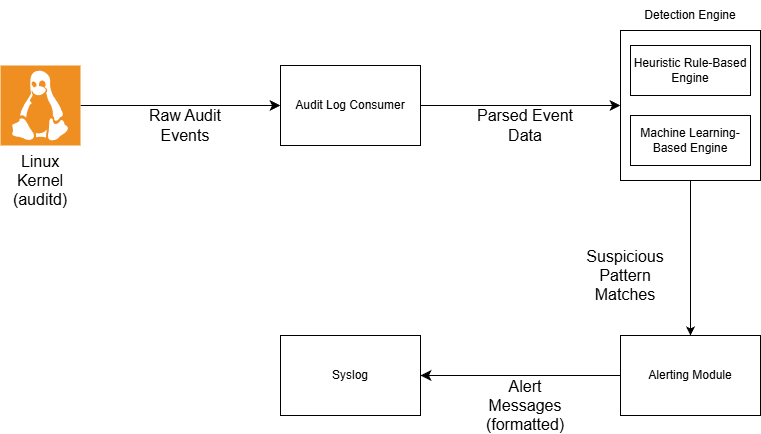
\includegraphics[width=1.0\linewidth]{CyberSP3.1.drawio (1).png}
    \caption{System architecture of the NoEsc daemon}
    \label{fig:architecture}
\end{figure}

The daemon's C++ core receives a real-time stream of audit events via the \texttt{audispd} plugin interface and parses them into structured \texttt{LogEvent} records. These records are then dispatched to two parallel paths:

\begin{enumerate}
    \item \textbf{Rule Engine Path:} The heuristic rule-based engine evaluates each event in-process using deterministic logic.
    \item \textbf{ML Bridge Path:} A non-blocking Unix Domain Socket (UDS) bridge forwards serialized JSON events to an external Python-based ML listener process for statistical classification.
\end{enumerate}

The UDS bridge uses a fire-and-forget datagram design (\texttt{SOCK\_DGRAM}) to ensure the rule engine path is never blocked by ML processing latency. It implements lazy initialization, rate-limited offline logging (60-second cooldown), and automatic recovery when the ML listener restarts.

To enable controlled experimentation, the daemon supports runtime engine mode selection via CLI flags (\texttt{--ml-only}, \texttt{--rules-only}) or the \texttt{NOESC\_ENGINE\_MODE} environment variable, allowing isolated evaluation of each engine on identical input streams. Additionally, the daemon provides an offline export mode (\texttt{--dump-json}) that serializes parsed events as newline-delimited JSON to \texttt{stdout}, used to generate ML training datasets with the same parser and contaminant filters applied in live detection, ensuring train-serve parity.

\subsection{Data Collection: The Linux Audit Framework}
The starting point of the detector is the native Linux Audit framework, chosen for its deep kernel-level visibility and universal availability \cite{groenewoud2024}. This will function as the single, unified Audit Log Consumer module for the entire system. Its primary function is to receive a real-time stream of events from the audit daemon and parse them into a structured format suitable for use by both the rule-based and machine learning Detection Engines.

\subsection{Audit Rule Configuration}
The system architecture prioritises low performance overhead so the system will not ingest all system logs. Instead, it will rely on a minimal and specified set of audit rules defined in \texttt{/etc/audit/rules.d/}. Following industry best practices for detection engineering \cite{groenewoud2024}, these rules will be configured to specifically monitor high-value events indicative of privilege escalation. The configuration is based on three main strategies:

\begin{enumerate}
    \item \textbf{Critical System Call Monitoring:} Rules will trace the most critical system calls related to program execution and privilege changes. For example:
    \begin{itemize}
        \item \texttt{-a always,exit -F arch=b64 -S execve -k weird\_exec}
        \item \texttt{-a always,exit -F arch=b64 -S setuid,setgid -k weird\_change}
    \end{itemize}

    \item \textbf{Sensitive File Integrity Monitoring:} The file-watch flag (\texttt{-w}) will be used to monitor for any write or attribute change permissions (\texttt{-p wa}) on files critical to user privileges. For example:
    \begin{itemize}
        \item \texttt{-w /etc/passwd -p wa -k weird\_identity\_change}
        \item \texttt{-w /etc/sudoers -p wa -k weird\_sudo\_change}
    \end{itemize}

    \item \textbf{Efficient Log Filtering:} All rules will be tagged with a unique key using the \texttt{-k} flag (e.g., \texttt{weird\_exec}, \texttt{weird\_identity\_change}). This allows the user-space daemon to subscribe only to tagged events, significantly filtering the log stream and ensuring the detector only processes relevant events \cite{groenewoud2024}.
\end{enumerate}

\subsection{Log Consumption and Parsing}
As for the log consumption, our detector will avoid the common but inefficient practice of using the \texttt{/var/log/audit/audit.log} file. Instead, the Audit Log Consumer will be implemented as a plugin for the \texttt{audispd} (audit dispatcher) framework. This approach is a key component of modern detection engineering, as it avoids the performance and latency issues associated with file-based log monitoring \cite{groenewoud2024}.

The audispd framework allows the auditd daemon to forward events directly to our detector process in real-time, which lowers the performance overhead and ensures that suspicious behavior of the attacks are analyzed as they occur. By creating such a plugin, the detector can receive security events faster. Upon receiving a raw log string, the consumer first parses it into a structured data format, extracting the key fields required by the Detection Engine. These fields, which provide the semantic information for both detection engines, are detailed in Table \ref{tab:audit_fields}.

\begin{table}[h]
    \centering
    \caption{Parsed audit event fields used by both detection engines}
    \begin{tabular}{|l|p{6cm}|}
        \hline
        \textbf{Field Name} & \textbf{Description} \\ \hline
        \texttt{type} & The type of the audit record (e.g., \texttt{SYSCALL}, \texttt{USER\_AUTH}). \\ \hline
        \texttt{syscall} & The name of the system call being executed (e.g., \texttt{execve}, \texttt{setuid}). \\ \hline
        \texttt{res} & The result field indicating success or failure of the event. \\ \hline
        \texttt{auid} & The Audit User ID, representing the original user who logged in. \\ \hline
        \texttt{euid} & The Effective User ID, representing the privileges the process is running with. \\ \hline
        \texttt{exe} & The full path to the executable that was run. \\ \hline
        \texttt{pid} & The Process ID of the event's subject. \\ \hline
        \texttt{timestamp} & The epoch timestamp of the audit event. \\ \hline
        \texttt{key} & The audit rule key tag that triggered the event. \\ \hline
    \end{tabular}
    \label{tab:audit_fields}
\end{table}

\subsection{Detection Engine: Rule-Based Behavioral Analysis}
The first of these two detection engines is heuristic and rule-based. This engine provides the starting line for this comparative study and represents a more traditional, fully transparent approach to threat detection. Its design emphasizes interpretability, where each alert can be reduced to a simple, human-readable rule. This is argued by Liu et al. (2021) where the focus on interpretability is the key point of rule-based systems, which makes them more "trustworthy" and for easier validation for an administrator \cite{liu2021}. This engine is stateful, designed to correlate a targeted stream of audit events over time to identify behavioral patterns indicative of privilege escalation.

The engine works by keeping an in-memory lightweight model of the system state, tracking mainly user activity scores. Every time new, relevant audit events come in from the Audit Log Consumer, it runs them through the heuristic rules. Whenever an event or a sequence of events triggers a rule's condition, the engine marks it as a potential threat and sends the Alerting Module a notification.

To demonstrate its capabilities, the prototype is implemented with the detection logic of three different and impactful privilege escalation vectors, namely SUID/SGID abuse, sudo misuse, and sensitive file tampering. These vectors were selected because they represent the most common misconfiguration-based attacks in modern Linux privilege escalation benchmarks \cite{happe2024}. This set proves that the engine can handle various types of detection logic: stateless heuristics, stateful scoring, and simple pattern matching.

The SUID path whitelist is externalized to a configuration file (\texttt{suid\_whitelist.conf}), allowing administrators to add trusted paths without recompiling. Full rule externalization to a JSON/YAML schema remains a design goal for future work.

\subsection{SUID/SGID Execution Analysis}
This module detects the abuse of programs misconfigured with the SUID or SGID bit, a common privilege escalation vector \cite{happe2024}. A simple rule that alerts on every SUID execution would generate unacceptable false positives from legitimate software (e.g., \texttt{passwd}). The implementation uses a \textbf{strict whitelist} approach: any SUID execution from a path not explicitly trusted is flagged.

Each \texttt{execve} system call is analyzed, and an alert is generated only if all of the following conditions are met:

\begin{enumerate}
    \item The Audit User ID (\texttt{auid}) belongs to a non-root user.
    \item The resulting Effective User ID (\texttt{euid}) of the new process is 0 (root).
    \item The executable's path (\texttt{exe}) is \textbf{not} within any trusted directory. The default whitelist includes: \texttt{/bin}, \texttt{/usr/bin}, \texttt{/sbin}, \texttt{/usr/sbin}, \texttt{/usr/lib}, \texttt{/usr/libexec}. An academic sandbox path (\texttt{/opt/student\_sandbox/}) is also whitelisted to accommodate supervised coursework.
\end{enumerate}

The whitelist approach is more secure than a blacklist because any novel attack path is detected by default. Two additional mechanisms reduce alert fatigue:
\begin{itemize}
    \item \textbf{Path-based severity classification:} Executables in high-risk directories (\texttt{/tmp/}, \texttt{/dev/shm/}) generate \texttt{CRITICAL} alerts, while executables in ambiguous paths (e.g., \texttt{/home/}) generate \texttt{WARNING} alerts.
    \item \textbf{Per-user cooldown:} A 10-second per-user cooldown prevents alert flooding from repeated \texttt{execve} events.
\end{itemize}

\subsection{Stateful Detection of Sudo Abuse}
This module addresses attacks that take advantage of overly permissive sudo rules \cite{happe2024}. A single \texttt{sudo} command can be legitimate, but a rapid succession of privileged commands is suspicious. This module is stateful, detecting suspicious behavior over time using a scoring mechanism, as shown in \textbf{Figure~\ref{fig:sudo_flowchart}}.

The engine maintains an in-memory hash map tracking the score for each user (\texttt{auid}). An \textbf{exec-only scoring gate} ensures that only process launch events (\texttt{execve}) increment the score, preventing follow-up syscalls from the same command from inflating scores. The scoring rules are:

\begin{enumerate}
    \item On \texttt{USER\_AUTH} failure events (\texttt{res=failed}): increment the user's score by +1.
    \item On a successful sudo execution of a high-risk command: increment the user's score by +5.
\end{enumerate}

High-risk commands include file manipulation utilities (\texttt{cp}, \texttt{tee}), permission-changing commands (\texttt{chmod}, \texttt{chown}), and system service management (\texttt{systemctl}). The +5 increment was calibrated to reduce false positives in the academic lab environment, where students frequently use \texttt{sudo apt} during coursework.

The engine uses \textbf{progressive alerting} with two thresholds: a \texttt{WARNING} alert at 15 points and a \texttt{CRITICAL} alert at 20 points. Scores decay after 60 seconds of inactivity. \textbf{Burst episode aggregation} is applied: the first \texttt{CRITICAL} alert in a burst is delivered immediately, while subsequent alerts are suppressed and summarized when the episode ends. A \textbf{maintenance mode} TTL allows operators to suppress \texttt{SudoMisuse} notifications during planned maintenance windows.

\begin{figure}[H]
    \centering
    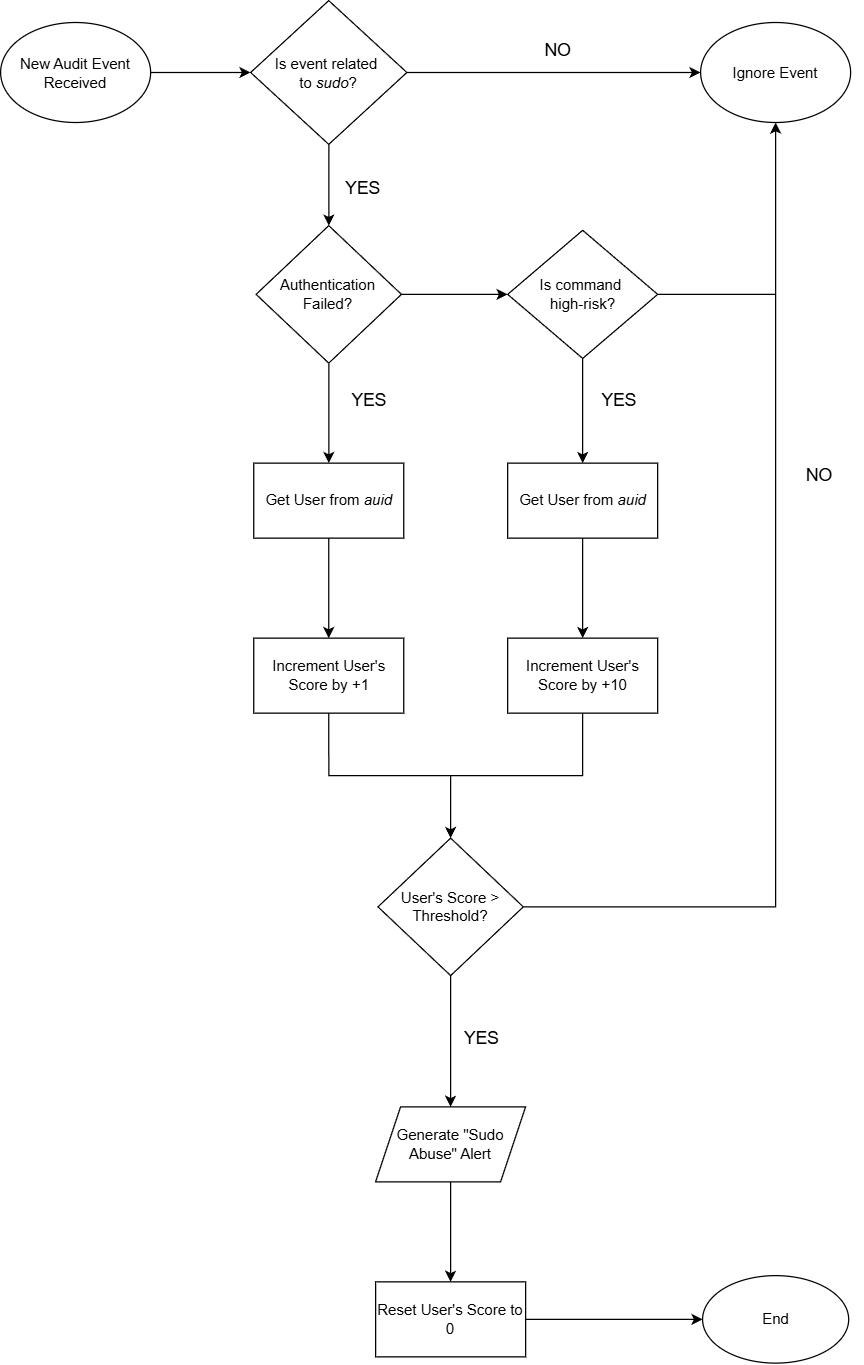
\includegraphics[width=0.85\linewidth]{Flowchart of the Stateful Sudo Abuse Detection Logic.drawio (2).png}
    \caption{Flowchart of the Stateful Sudo Abuse Detection Logic}
    \label{fig:sudo_flowchart}
\end{figure}

\subsection{Sensitive File Tampering}

This module detects unauthorized attempts to modify critical files that control user privileges. The detection leverages the audit system's file-watch (\texttt{-w}) rules, which tag events with keys such as \texttt{identitychange} (for \texttt{/etc/passwd}, \texttt{/etc/shadow}) and \texttt{sudochange} (for \texttt{/etc/sudoers}).

An alert is generated when an audit event carries one of these watch keys and the process's \textbf{Effective User ID} (\texttt{euid}) is \textbf{not 0} (i.e., not root). This logic reflects the correct threat model: modifications to these critical files should only be performed by the root user, so any non-root process attempting modification indicates a malicious tampering attempt. Events where \texttt{euid=0} are suppressed, as they represent authorized administrative actions.

\subsection{Alerting Architecture}
The daemon implements a four-tier alert delivery system to serve different operational contexts:

\begin{enumerate}
    \item \textbf{STDERR:} Real-time console output for manual testing and debugging.
    \item \textbf{Persistent File:} All alerts are appended to \texttt{/var/log/noesc\_alerts.log} for forensic review.
    \item \textbf{Syslog:} Alerts are forwarded to the system's \texttt{LOG\_AUTH} syslog facility for integration with enterprise SIEM tools (e.g., journald, rsyslog).
    \item \textbf{Desktop Notifications:} Visual alerts via \texttt{gdbus} for \texttt{CRITICAL} severity events, with a 150ms inter-notification delay to prevent stacking.
\end{enumerate}

Each alert is severity-labeled (\texttt{WARNING} or \texttt{CRITICAL}) and includes the attack vector, affected user, process details, and an \texttt{ausearch} command referencing the event's audit serial number for immediate forensic investigation.
\subsection{Detection Engine: Machine Learning-Based Behavioral Analysis}
The second detection engine involves more of a data-driven approach in contrast to the heuristic and rule-based approach earlier. This engine utilizes machine learning in detecting anomalies in the auditd system, classifying them according to normalcy, or of malicious activity, which is normal in intrusion detection systems. Picking a model suitable in finding malicious activity is essential as it affects the success rate, accuracy, and correctness of the results. 

Each of the models has their own advantages and disadvantages. While ensemble methods like Random Forest (RF) are often cited for their potential interpretability, this quality diminishes as model complexity increases to handle real-world data, rendering them effective ``black boxes'' in practice \cite{pereira2018}. Given that both high-performing SVM and RF models are functionally opaque, this study prioritizes the model with the highest demonstrated accuracy for the specific task of host-based intrusion detection. Comparative analyses have shown Support Vector Machine (SVM) to achieve superior accuracy over RF in this domain \cite{kumar2023}, with a particularly strong ability to correctly classify benign system activity \cite{shin2020}. Therefore, based on its established high accuracy for this task, this engine will utilize SVM as its core classification model.

\subsection{Feature Engineering Pipeline}\label{sec:feature-pipeline}
The main challenge of the ML approach is feature engineering---transforming raw data into information suitable for machine learning. System call traces are treated as text, applying NLP techniques---a common methodology in HIDS research \cite{zhang2020, khandelwal2022}.

The implemented pipeline consists of two stages:
\begin{enumerate}
    \item \textbf{N-gram Generation and TF-IDF Vectorization:} A sliding window generates overlapping (2,3)-gram sequences of system call tokens. These are transformed into numerical vectors using TF-IDF, weighting n-grams that are characteristic of malicious behavior \cite{zhang2020}.
    \item \textbf{Contextual Feature Augmentation:} Eight contextual features are appended to each TF-IDF vector to capture privilege and authentication context not visible in syscall sequences alone. These features are defined in a shared feature contract (version \texttt{v2\_syscall\_user\_auth\_context}) to ensure train-serve parity.
\end{enumerate}

The contextual features are:
\begin{itemize}
    \item \texttt{ctx\_euid\_is\_root}: whether any event in the sequence has \texttt{euid=0}.
    \item \texttt{ctx\_auid\_euid\_mismatch}: whether any event shows \texttt{auid $\neq$ euid} (a privilege change indicator).
    \item \texttt{ctx\_exe\_in\_tmp}: whether any executable path starts with \texttt{/tmp/} or \texttt{/dev/shm/}.
    \item \texttt{ctx\_auth\_failure\_rate}: the ratio of failed to total \texttt{USER\_AUTH} events in the sequence.
\end{itemize}

Recursive Feature Elimination (RFE), proposed in the original design, was not implemented. The (2,3)-gram TF-IDF with contextual features provided sufficient discrimination (MCC = 0.995 on the primary model) without the computational overhead of RFE.

\subsection{Model Training and Classification}
Labeled datasets were constructed using a hybrid approach. Benign data was collected directly from workstations in the ICS computer laboratories to capture authentic student usage patterns, while malicious data was generated by executing the attack scripts detailed in \textbf{Section~\ref{sec:test-scenarios}} within a controlled environment. Raw audit logs were exported using the daemon's \texttt{--dump-json} mode to ensure the same parser and contaminant filters are applied during both training and live inference.

Events are grouped by \texttt{(source\_file, pid)} to form process-local syscall sequences. A \textbf{minimum events per sequence} gate filters out sequences shorter than a configurable threshold, removing noise from trivially short process lifetimes. The dataset is split chronologically (70\% train, 30\% test) with no random shuffling, preserving temporal validity. The SVM classifier uses a linear kernel with balanced class weights and a fixed random state of 42 for reproducibility.

\subsubsection{Dual-Model Architecture}
A key finding during development was that sequences with only 1--2 syscall events lack sufficient behavioral context for reliable classification. Rather than discarding these short sequences entirely, the system implements a \textbf{dual-model architecture}:

\begin{itemize}
    \item \textbf{Long model} (v4, \texttt{min\_events=3}): Handles sequences with $\geq$3 events. This is the primary classifier.
    \item \textbf{Short model} (short\_v1, \texttt{min\_events=1}): Purpose-built for sequences with 1--2 events, trained on a dedicated short-window dataset.
\end{itemize}

At runtime, the ML listener routes each sequence to the appropriate model based on its length. Short-model predictions are subject to a \textbf{score-based demotion threshold}: predictions classified as malicious but with a decision function score below a configurable threshold are demoted to benign, reducing false positives from ambiguous short sequences.

\subsection{Capturing Privilege Escalation Events in \texttt{auditd}}
To effectively design both detection engines, it is essential to understand how a privilege escalation attack is captured by the \texttt{auditd} data source. This single source of truth provides distinct types of signals that are consumed differently by the heuristic and machine learning approaches.

As a concrete example, consider the common SUID binary abuse vector where an attacker executes a privileged shell from a world-writable directory: \texttt{/tmp/sh -p}. The \texttt{auditd} rule monitoring the \texttt{execve} system call will capture this event, generating a log entry similar to the following:

\begin{verbatim}
type=SYSCALL msg=audit(...): 
arch=c000003e syscall=59 exe="/tmp/sh" 
auid=1001 uid=1001 euid=0 key="priv_exec"
\end{verbatim}

This single event provides crucial evidence for both engines, but is interpreted in fundamentally different ways:

\subsubsection*{For the Heuristic Rule-Based Engine}
The rule-based engine interprets this log as a set of explicit, human-readable facts. It directly parses the fields and applies its deterministic logic:
\begin{itemize}
    \item The field \texttt{auid=1001} confirms the action was initiated by a non-root user.
    \item The field \texttt{euid=0} confirms that the process successfully gained root privileges.
    \item The field \texttt{exe="/tmp/sh"} confirms the execution occurred from a non-standard, suspicious path.
\end{itemize}
Because all three conditions of the predefined rule are met, the engine identifies this event as a high-confidence malicious act. It is an explicit signal.

\subsubsection*{For the Machine Learning-Based Engine}
The machine learning engine does not interpret the semantic meaning of the fields. Instead, it treats the event as a statistical component within a sequence.
\begin{itemize}
    \item The most critical piece of information is the system call number, represented by \texttt{syscall=59}. This number becomes a single "word" in a long "document" representing the process's execution trace.
    \item This "word" is then analyzed as part of a sequence (an n-gram). The feature engineering pipeline may discover that the n-gram representing, for example, \texttt{open -> chmod -> execve} is a very rare and high-weight feature according to its TF-IDF calculation.
    \item The SVM classifier, having been trained on thousands of examples, has learned that the presence of this specific, high-weight statistical pattern strongly correlates with malicious activity.
\end{itemize}
For the ML engine, the log is not an explicit fact but a statistical signal that contributes to a larger, learned pattern of behavior. This section's example illustrates how both methodologies, while using the same raw data, operate on different principles to achieve the same goal.

\subsection{Development Tools}
All experiments will be conducted in a controlled and reproducible virtualized environment, configured with the following specifications:

\begin{itemize}
    \item \textbf{Host Environment:} The host machine will be a university laboratory computer (ICS, UPLB) with a 13th Gen Intel Core i5-13400 processor and 16 GB of RAM.
    
    \item \textbf{Guest Environment:} All tests will run within a VirtualBox guest virtual machine running Ubuntu 22.04 LTS Server Edition. The VM will be allocated 2 virtual CPUs and 4 GB of RAM to simulate a typical, non-specialized Linux host.
    
    \item \textbf{Implementation Stack:} The rule-based engine will be implemented in C++. The machine learning engine will be implemented in Python 3 using the \texttt{pandas} and \texttt{scikit-learn} libraries.
    
    \item \textbf{System Configuration:} Both detector prototypes will be deployed as background \texttt{systemd} services. A single, consistent set of audit rules will be defined in a custom file (\texttt{sp-detector.rules}) to provide an identical stream of events to both engines.
    
    \item \textbf{Reproducibility:} To ensure repeatability, all attack scenarios and benign workloads will be executed using automated Bash scripts.
\end{itemize}

\subsection{Test Scenarios}\label{sec:test-scenarios}
% --- BEGIN SIMPLIFIED INTRO ---
Both detection engines will be evaluated against three distinct test scenarios drawn from the "Got Root?" benchmark to ensure they represent common, real-world privilege escalation vectors \cite{happe2024}. For consistency, each test will be executed via an automated Bash script.
% --- END SIMPLIFIED INTRO ---

\subsubsection{\textbf{Benign Workload Simulation}}
To simulate the typical usage patterns of a Computer Science student in a laboratory setting and generate training data for the ML model, a benign workload script will be executed. This script automates common development tasks, including:

\begin{itemize}
    \item \textbf{Files:} Navigating directories, creating/deleting files, and using editors like \texttt{vim} and \texttt{nano}.
    \item \textbf{Compilation:} Compiling C or C++ programs using \texttt{gcc}.
    \item \textbf{Package Management:} Installing, updating, or removing packages using \texttt{apt} or other package managers.
\end{itemize}
This scenario serves as the baseline for performance benchmarking and the source of "normal" data for ML training.

\subsubsection{\textbf{Test Case 1 (SUID Binary Abuse)}}
The first scenario will be SUID Binary Abuse. To set this up, the test script places a copy of \texttt{/bin/bash} into the \texttt{/tmp/} directory and applies the SUID permission bit. It then simulates an attacker executing this misconfigured binary from the untrusted location. This tests the engine's ability to apply a stateless heuristic, correlating the process execution (\texttt{execve} syscall) with its untrusted path and its elevated privileges (\texttt{euid=0}).

\subsubsection{\textbf{Test Case 2 (Stateful Sudo Misuse)}}
The second scenario will evaluate the detection of \texttt{sudo} abuse through stateful analysis. The test environment will be configured with a \texttt{sudoers} rule that requires a password for the test user account. A script will then simulate a brute-force attack by making ten consecutive, incorrect \texttt{sudo} password entries in a loop. This scenario is designed to test the stateful capabilities of the detection engine.

\subsubsection{\textbf{Test Case 3 (Sensitive File Tampering)}}
The final scenario will test the engine's high-confidence pattern matching for file integrity. A file-watch rule for the \texttt{/etc/passwd} file will be active in the \texttt{auditd} configuration. The test will be executed by a script, running as a non-root user, that attempts to append a new user entry to this critical file. This scenario validates the engine's ability to immediately flag unauthorized write attempts on sensitive system files.

\subsection{Rule-Based Engine Metrics}
The logic of the heuristic rule-based engine is deterministic, as it forms the basis for a fixed set of predefined rules. Hence, the main objective of the heuristic rule-based engine evaluation should be to ensure that it is effective in catching what it is supposed to catch and it does not flag what it is not supposed to flag. The two most important metrics in this regard would then be the True Positive Rate and the False Positive Rate.

The objective measure of success will be 100\% TPR against the attack scenarios targeted. For each of the three test cases, the engine producing the specific alert required in the system log is defined as a successful detection. A failure to produce the expected alert constitutes a False Negative.

This would be further validated by the Benign Workload Test  for the measurement of the False Positive Rate. The aim for such a test is zero FPR; no alerts from the detector in normal operation.

\subsection{Machine Learning Engine Metrics}
Similar to the rule-based engine, the machine learning engine will be evaluated with labels Detected/Not detected. The engine is tasked into classifying between real and malicious system activity. The methodology for the machine learning engine follows the standard way in machine learning research.

First, construction of the labeled dataset is necessary. The dataset will be composed of data from two distinct sources. The dataset for malicious activity will be generated by continuously repeating the attack scenarios indicated in the test cases. Conversely, safe (benign) data will be obtained by gathering system events from live laboratory computers during regular usage hours. This includes actual student activities such as, but not limited to, compiling software, accessing development tools, and managing files, providing a rigorous real-world baseline.

Second, feature engineering is a must and its process will be designed to convert the raw auditd logs into useful information that is suitable for the model. This process will get the needed attributes from the events such as the syscall name, user IDs (\texttt{auid}, \texttt{euid}), executable paths, and the frequency of security-sensitive events within a certain period of time.

Lastly, the dataset that we have obtained will be split into a training and testing set. After training the model on the training data, its performance will be measured using our testing data. The results will be shown using a confusion matrix, and its primary metrics for success will be:r
\begin{enumerate}
    \item \textbf{Recall} is the proportion of actual positive cases (attacks) that are correctly identified as positive. It is computed by:
    \[
    Recall = \frac{TP}{TP + FN}
    \]
    
    \item \textbf{Precision} is the proportion of positive predictions that were actually correct. It is computed by:
    \[
    Precision = \frac{TP}{TP + FP}
    \]
    
    \item \textbf{F1-Score} is the harmonic mean of precision and recall, providing a balance between the two metrics. It is computed by:
    \[
    F1\text{-}Score = \frac{2 \times Recall \times Precision}{Recall + Precision}
    \]

    \item \textbf{Accuracy} is the overall proportion of correct predictions (both positive and negative) out of the total number of cases. It is computed by:
    \[
    Accuracy = \frac{TP + TN}{TP + TN + FP + FN}
    \]

\end{enumerate}
where $TP$ is True Positive, $TN$ is True Negative, $FP$ is False Positive, and $FN$ is False Negative.

Sometimes, data can also be highly imbalanced as intrusion detection datasets cannot really account for a suitable number of benign and malicious data (e.g: unequal number of benign events to malicious events). Thus, the study will use two further metrics: 

\begin {itemize}
\item \textbf{Area Under the ROC Curve (AUC)} - used to assess the model's overall ability to distinguish between malicious and benign activity. \cite{shin2020}
\item \textbf{Matthews Correlation Coefficient (MCC)} - to provide a single, imbalanced score of classification quality that is reliable even on imbalanced data. \cite{jiang2024} 
\end{itemize}

\subsection{Performance Overhead Benchmarking}
Performance overhead was evaluated using two complementary benchmarks: a macro benchmark measuring the system-level cost of the audit rules, and a micro benchmark measuring the raw throughput capacity of the ML engine. This distinction is important because NoEsc's C++ daemon operates as a passive \texttt{audispd} consumer and does not intercept system calls in the kernel path. Therefore, the primary source of overhead attributable to NoEsc is the set of kernel-level audit rules that must be active for the system to observe events.

\subsubsection{Macro Benchmark: Audit Rule Overhead}
The macro benchmark quantifies the overhead imposed by loading NoEsc's audit rules into the kernel. The workload is the compilation of the NoEsc daemon itself (\texttt{make clean \&\& make}), a CPU- and I/O-intensive task that generates a high volume of the exact syscall types monitored by the rules (e.g., \texttt{execve}, \texttt{chmod}). Wall-clock build time was recorded over five trials under two conditions: (1) a \textbf{Baseline} with all NoEsc audit rules flushed from the kernel, and (2) \textbf{With NoEsc Rules}, where the full \texttt{99-noesc.rules} ruleset was active. The percentage overhead was calculated as the relative increase in average build time from the baseline condition.

\subsubsection{Micro Benchmark: ML Engine Throughput}
The micro benchmark measures the raw event ingestion and classification capacity of the Python ML listener. A synthetic audit event representative of a privilege escalation attempt was constructed and sent to the ML engine's Unix Domain Socket (UDS) in a tight loop of 10,000 events. Throughput is reported in Events Per Second (EPS), directly quantifying how many sequences the ML pipeline can score per second and establishing whether the engine can sustain the event rates observed in a live system.

% RESULTS AND DISCUSSION
\section{Results and Discussion}

\subsection{Machine Learning Model Performance}

Multiple SVM model variants were trained to evaluate the impact of dataset composition and the minimum events per sequence parameter. Table~\ref{tab:model_comparison} summarizes the performance of all trained models on their respective test sets.

\begin{table}[H]
    \centering
    \footnotesize
    \setlength{\tabcolsep}{3pt}
    \renewcommand{\arraystretch}{1.1}
    \caption{SVM Model Performance Comparison}
    \begin{tabular}{|l|c|c|c|c|c|c|}
        \hline
        \textbf{Model} & \textbf{min} & \textbf{Acc} & \textbf{Prec} & \textbf{Rec} & \textbf{F1} & \textbf{MCC} \\ \hline
        v1             & 2   & .968 & .971 & .991 & .981 & .894 \\ \hline
        v3             & 3   & .952 & .906 & 1.00 & .951 & .908 \\ \hline
        v4 (min2)      & 2   & .795 & .999 & .765 & .867 & .543 \\ \hline
        \textbf{v4 (min3)} & \textbf{3} & \textbf{.998} & \textbf{.998} & \textbf{.999} & \textbf{.998} & \textbf{.995} \\ \hline
        short\_v1      & 1   & .821 & .960 & .663 & .785 & .672 \\ \hline
    \end{tabular}
    \label{tab:model_comparison}
\end{table}

The v4 model with \texttt{min\_events=3} achieves the highest overall performance (F1 = 0.998, MCC = 0.995), demonstrating near-perfect classification on the university lab dataset. The \texttt{min\_events\_per\_sequence} parameter proved to be the most impactful hyperparameter: filtering out short sequences (1--2 events) dramatically improved recall from 0.765 to 0.999 on the same dataset, as short sequences lack sufficient behavioral context for reliable classification.

The short\_v1 model, purpose-built for sequences with 1--2 events, achieves lower but serviceable performance (F1 = 0.785). Its lower recall (0.663) reflects the inherent ambiguity in classifying processes with minimal syscall traces.

\subsubsection{Negative Control Validation}
To validate that the model's discriminative power comes from genuine signal rather than data artifacts, a negative control experiment was conducted by training on a dataset where both the ``benign'' and ``malicious'' classes contained only benign data. The result (Accuracy = 0.500, MCC = 0.000) confirms that the model learns no signal from identical distributions, ruling out label leakage as a confounding factor.

\subsection{Rule-Based Engine Evaluation}

The rule engine is deterministic---given identical input, it produces identical output. Its evaluation is therefore binary: each test vector either triggers the expected alert or it does not. Table~\ref{tab:rules_eval} summarizes the results.

\begin{table}[H]
    \centering
    \footnotesize
    \setlength{\tabcolsep}{3pt}
    \renewcommand{\arraystretch}{1.1}
    \caption{Rule-Based Engine Detection Results}
    \begin{tabular}{|l|p{3cm}|l|l|}
        \hline
        \textbf{Vector} & \textbf{Scenario} & \textbf{Exp.} & \textbf{Res.} \\ \hline
        SUID & \texttt{/tmp/backdoor} & CRIT & TP $\checkmark$ \\ \hline
        SUID & \texttt{/home/.../myshell} & WARN & TP $\checkmark$ \\ \hline
        SUID & \texttt{/opt/sandbox/} & None & TN $\checkmark$ \\ \hline
        Sudo & 4 cmds + auth fail & W+C & TP $\checkmark$ \\ \hline
        File & Non-root $\rightarrow$ \texttt{shadow} & CRIT & TP $\checkmark$ \\ \hline
        File & Root $\rightarrow$ \texttt{shadow} & None & TN $\checkmark$ \\ \hline
        Benign & \texttt{sudo apt update} & None & TN $\checkmark$ \\ \hline
    \end{tabular}
    \label{tab:rules_eval}
\end{table}

The rule engine achieved 100\% True Positive Rate on all targeted attack scenarios and 0\% False Positive Rate on the benign workload, meeting the design objectives outlined in the methodology.

\subsection{Fairness Comparison: ML-only vs Rules-only}

To compare the two engines fairly, the same mixed audit log (90,713 benign events from a real university lab capture combined with 22 hand-crafted attack events covering all three vectors) was replayed through each engine independently across three repeated runs. Table~\ref{tab:fairness} summarizes the results.

\begin{table}[H]
    \centering
    \footnotesize
    \setlength{\tabcolsep}{4pt}
    \renewcommand{\arraystretch}{1.1}
    \caption{Fairness Comparison: Alert Volume (3-run avg.)}
    \begin{tabular}{|l|c|c|}
        \hline
        \textbf{Metric} & \textbf{ML} & \textbf{Rules} \\ \hline
        Mean alerts & 108.00 & 7.00 \\ \hline
        Alert rate (\%) & 0.119 & 0.008 \\ \hline
        Per-run range & 88--121 & 7/7/7 \\ \hline
        WARNING & --- & 2.00 \\ \hline
        CRITICAL & --- & 5.00 \\ \hline
    \end{tabular}
    \label{tab:fairness}
\end{table}

The rules engine is perfectly deterministic (7 alerts across all runs, zero variance), producing exactly one alert per injected attack event. The ML engine generates approximately 15$\times$ more alerts, with natural variance (88--121) arising from timing-dependent PID buffer management and sequence boundary effects during live replay.

The higher ML alert count is not primarily caused by insufficient training data. Rather, it reflects a fundamental architectural difference: the rule engine evaluates each event against three narrow, hardcoded patterns, while the ML engine classifies \textit{every} PID-grouped syscall sequence (approximately 4,900 sequences per run). Even with the v4 model's low FPR of 0.4\%, applying it to thousands of sequences produces dozens of false positives from legitimate system processes (e.g., \texttt{snap-update-ns}, \texttt{cron}, \texttt{xtables-nft-multi}) whose syscall patterns resemble attack signatures in the TF-IDF feature space.

\subsection{Performance Overhead Benchmarking}

\subsubsection{Macro Benchmark: Audit Rule Overhead}
The macro benchmark measured the wall-clock compilation time of the NoEsc daemon itself across five trials under two conditions. Table~\ref{tab:macro_bench} summarizes the results.

\begin{table}[H]
    \centering
    \footnotesize
    \setlength{\tabcolsep}{4pt}
    \renewcommand{\arraystretch}{1.1}
    \caption{Macro Benchmark: Build Time Overhead (5-run avg.)}
    \begin{tabular}{|l|c|c|}
        \hline
        \textbf{Condition} & \textbf{Avg. Build Time (s)} & \textbf{Overhead} \\ \hline
        Baseline (no audit rules) & 3.5550 & --- \\ \hline
        With NoEsc rules active   & 3.5556 & +0.02\% \\ \hline
    \end{tabular}
    \label{tab:macro_bench}
\end{table}

The measured overhead of \textbf{0.02\%} is negligible, confirming that the NoEsc audit ruleset imposes no meaningful performance cost on a live system. This result is consistent with the architectural rationale: the NoEsc daemon operates as a passive \texttt{audispd} consumer and does not intercept system calls in the kernel path. The kernel audit framework handles event generation asynchronously, so the only cost of enabling the rules is the additional log buffer entries generated by the monitored syscall types (\texttt{execve}, \texttt{chmod}, \texttt{chown}).

\subsubsection{Micro Benchmark: ML Engine Throughput}
The micro benchmark measured the raw event ingestion capacity of the Python ML listener by sending 10,000 synthetic audit events over the Unix Domain Socket. The listener processed the full batch in \textbf{0.248 seconds}, yielding a throughput of approximately \textbf{40,393 Events Per Second (EPS)}. For reference, the live system captured a benign-workload log of 90,713 events over a multi-hour university lab session, representing a sustained rate well below 1 EPS in real-world conditions. The ML engine's throughput capacity therefore provides substantial headroom, confirming that the Python inference pipeline is not a bottleneck under realistic deployment conditions.

\subsection{Comparative Analysis}


Table~\ref{tab:comparison} synthesizes the findings across the evaluation dimensions.

\begin{table}[H]
    \centering
    \footnotesize
    \setlength{\tabcolsep}{3pt}
    \renewcommand{\arraystretch}{1.1}
    \caption{Comparative Analysis of Detection Engines}
    \begin{tabular}{|p{1.5cm}|p{2.5cm}|p{2.5cm}|}
        \hline
        \textbf{Criterion} & \textbf{Rule-based} & \textbf{ML Engine} \\ \hline
        Detection & 100\% TPR on 3 vectors; 0\% FPR & F1=.998; FPR=0.4\% \\ \hline
        Coverage & 3 hardcoded vectors only & Generalizes to unseen patterns \\ \hline
        Alerts & 7 (deterministic) & $\sim$108 (15$\times$ higher) \\ \hline
        Interpret. & High: human-readable & Low: statistical \\ \hline
        Extend. & Moderate: config + recompile & High: retrain \\ \hline
    \end{tabular}
    \label{tab:comparison}
\end{table}

\subsection{Discussion}

The results demonstrate a clear precision-coverage tradeoff between the two detection methodologies.

The rule-based engine achieves perfect detection on its targeted attack vectors with zero false positives, validating the interpretability advantage described by Liu et al. \cite{liu2021}. However, its coverage is inherently limited to the three vectors explicitly programmed. Any attack outside these patterns---such as a novel kernel exploit or a container escape---would go undetected.

The ML engine, by contrast, evaluates every process's behavior and can detect patterns not anticipated during development. This broader coverage comes at the cost of higher alert volume, which represents a practical concern for administrator alert fatigue in production deployments. The dual-model architecture and score-based demotion threshold partially mitigate this by reducing false positives from short sequences, but the fundamental tradeoff remains: statistical classification over thousands of sequences inevitably produces some false alerts from benign system processes whose behavior overlaps with attack patterns in the feature space.

For the specific context of an academic laboratory environment like the UPLB ICS labs, a hybrid approach---using the rule engine for high-confidence, immediate alerting on known vectors while the ML engine provides broader background monitoring---offers the most practical balance.

\subsection{Threats to Validity}

\begin{enumerate}
    \item \textbf{Weak labels:} Dataset labeling is directory-based (benign vs. malicious source directories), meaning some benign sequences may appear in malicious data and vice versa. The negative control experiment (MCC = 0.000 on benign-vs-benign) validates that the model learns genuine signal despite label noise.
    \item \textbf{Dataset bias:} All data was collected from UPLB ICS laboratories. Generalization to production environments with different workloads is not validated.
    \item \textbf{Temporal validity:} The chronological train/test split preserves temporal ordering, but the model may not generalize to future attack techniques not present in training data.
    \item \textbf{Single-site deployment:} All experiments were conducted on a single hardware configuration (13th Gen Intel i5, 16GB RAM). Performance characteristics may differ on other hardware.
    \item \textbf{RFE not implemented:} Recursive Feature Elimination, proposed in the original design, was not implemented. The (2,3)-gram TF-IDF with contextual features provided sufficient performance without it.
\end{enumerate}

% CONCLUSION AND FUTURE WORK
\section{Conclusion and Future Work}

\subsection{Conclusion}

This study designed, implemented, and comparatively evaluated two detection methodologies for privilege escalation on Linux: a heuristic rule-based engine and an SVM-based machine learning engine. The system was deployed as a lightweight, user-space daemon integrated with the native Linux Audit framework via the \texttt{audispd} plugin interface.

The rule-based engine achieved 100\% True Positive Rate on all three targeted attack vectors (SUID abuse, sudo misuse, and sensitive file tampering) with zero false positives, validating its suitability for high-confidence alerting on known threats. The machine learning engine, using the best-performing v4 model (F1 = 0.998, MCC = 0.995), demonstrated strong offline classification performance but produced approximately 15$\times$ more alerts than the rule engine when deployed on a mixed workload containing real university lab traffic.

This alert volume difference is not a deficiency of either approach but rather a manifestation of a fundamental precision-coverage tradeoff: the rule engine evaluates events against three narrow, deterministic patterns, while the ML engine classifies every process's behavioral sequence, inevitably producing false positives on benign system processes whose syscall patterns overlap with attack signatures in the TF-IDF feature space. This finding empirically demonstrates the tradeoff between interpretability and coverage that motivates hybrid detection architectures.

For the specific context of an academic laboratory environment, the hybrid approach---combining high-confidence rule-based alerting on known vectors with broader ML-based background monitoring---offers the most practical balance between detection coverage and administrator alert fatigue.

\subsection{Future Work}

Based on the experimental findings, several improvements are recommended to enhance the ML engine's precision in live deployment. The first of these was implemented as part of this study; the remainder are proposed as future extensions.

\begin{enumerate}
    \item \textbf{Process-Aware Whitelisting (Implemented).} An ML-level process whitelist was implemented to address the primary source of false positives: known system processes (e.g., \texttt{fuser}, \texttt{fusermount3}, \texttt{gdm-session-worker}, \texttt{snap}, \texttt{systemd-executor}) whose privileged syscall patterns resemble attack signatures. The whitelist is stored in a configuration file (\texttt{/etc/noesc/ml\_process\_whitelist.conf}) and supports both exact path matches and prefix-based matches. At runtime, the ML listener checks each process's executable path against the whitelist before inference, skipping whitelisted processes entirely. When evaluated on the same mixed workload, the whitelist reduced mean ML alerts from 89 to 28---a 68\% reduction---narrowing the ML-to-rules alert ratio from approximately 13:1 to 4:1 while preserving all true positive detections.

    \item \textbf{Larger and More Diverse Training Data.} All training data was collected from a single UPLB ICS laboratory site. Expanding the dataset to include benign activity from multiple environments (different lab configurations, server workloads, different academic semesters) would improve the model's generalization and reduce false positives on unfamiliar but legitimate system activity.

    \item \textbf{Recursive Feature Elimination (RFE).} RFE was proposed in the original design but not implemented due to the sufficient discrimination achieved by (2,3)-gram TF-IDF with contextual features. Applying RFE would prune noisy n-gram features that contribute to false positives, potentially improving precision without sacrificing recall \cite{patel2024}.

    \item \textbf{Calibrated Confidence Thresholds.} The current dual-model architecture uses a score-based demotion threshold for short sequences. Extending this approach to the primary model using Platt scaling would convert raw SVM decision scores into calibrated probabilities, enabling tiered alerting (e.g., high-confidence alerts for scores above 0.9, suppression below 0.7) and reducing alert fatigue.

    \item \textbf{Per-Process Feature Enrichment.} Augmenting the feature vector with process-level context---such as executable path classification (system binary vs.\ user-writable path), parent process identity, and user session type---would give the model stronger discriminative signals between legitimate privileged operations and actual privilege escalation attacks.

    \item \textbf{Online Incremental Learning.} The current model is static after training. An online learning approach that adapts to the specific host's behavioral baseline over time would allow the model to learn that a particular machine's recurring daemon patterns are benign, reducing false positives without manual intervention.
\end{enumerate}


% APPENDICES
% BIBLIOGRAPHY
\bibliographystyle{IEEEtran}
\bibliography{./cs190-ieee}

% BIOGRAPHY
\begin{biography}{Klenn Jakek V. Borja}
is a 4th year BS Computer
Science Student from the Institute of Computer Science, University of the Philippines Los Banos. His main research interests include cybersecurity and networking
\end{biography}


\end{document}
 
